\section{Sustainability}

In the following sections I'll discuss the different areas of the sustainability of 
the project. Said areas are: economical sustainability, social sustainability and 
environmental sustainability.

\subsection{Economical sustainability}

In this document we have assessed the various costs of the resources required for 
the completion of the project.

The project is, in its core, a tool for reducing the work for a game developer. Once 
the framework is done, any future adjustments or updates will most probably be linked 
to a new need for a feature of a future project. The framework has been designed to 
be easily extended so the cost of future extensions should not be highly affected 
by the fact that they are extensions of the framework.

The cost of the project is relatively low and, although was not thought to be directly 
profitable, it will most probably be amortized when developing games with it, as it 
reduces the development time of video-games.

The service that this project will offer to its user could also be obtained from all 
the other game engine and frameworks that already exist in the market and open-source 
repositories. What this project offers is a lower level solution for those users that 
want to hand-craft their game from scratch.

\subsection{Social sustainability}

Nowadays, there is a high interest in game development. The video-game industry has 
grown a lot and many small studios have appeared. There have also appeared a set of 
full, free game-engines that have allowed for those small studios, and even students, 
to rapidly produce fully fleshed out products.

In this context, where these game-engines abstract all the inner systems from the 
user, some people may find they've lost control or that they want to learn the insides 
of a game. This is where this projects comes in. It offers the bare minimum systems 
for a game to be: a main loop, an actor pool with behaviors and a extension system 
to allow the user of the framework to extend it however they want, using any technology 
they want.

The scope of this project doesn't just involve the main framework, but also a multimedia 
plug-in for it. Any future user of the product will see the implementation time of 
their game reduced by just needing to focus on the gameplay systems. Therefore, improving 
the life of the game developer using it.

\subsection{Environmental sustainability}

The resources required for this project are listed in the Budget estimation section 
of this document.

During the development of this project the only resource that will consume energy 
will be the Laptop PC. Assuming it is connected all the time to an electricity source 
and the charger consuming around 60W, through all the project it will consume approximately 
13kWh, which is roughly equivalent to 3,9 kg of CO2\cite{CO2}. It is not a high amount 
of energy and may be reused by taking advantage of the laptop's battery.

\subsection{Sustainability table}

Considering the contents of this document, I've come up with the following table:

\begin{figure}[H]
    \centering
    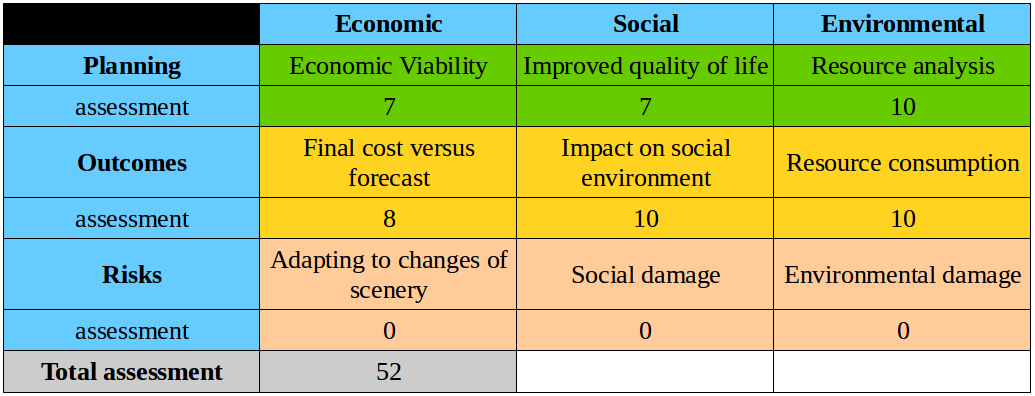
\includegraphics[width=\textwidth]{sustainability_table}
    \caption{Sustainability table}
    \label{fig:sustainability_table}
\end{figure}
